\documentclass[runningheads]{llncs}

\let\proof\relax
\let\endproof\relax
\usepackage{amsmath,amsthm,amssymb}
\usepackage{tikz, tikz-cd}

\newcommand{\A}{\mathcal{A}}
\newcommand{\G}{\mathcal{G}}
\renewcommand{\P}{\mathfrak{A}}
\newcommand{\C}{\mathfrak{C}(\Am,\e)}
\newcommand{\Z}{\mathbb{Z}}
\newcommand{\Q}{\mathbb{Q}}
\newcommand{\2}{\textbf{2}}
\newcommand{\Am}{\textbf{A}}
\newcommand{\del}{\partial}
\renewcommand{\v}{\bar{v}}
\newcommand{\e}{\bar{e}}
\newcommand{\T}{\mathcal{T}}

\newtheorem{thm}{Theorem}

\title{Extensions of Abelian Automata Groups}
\author{Chris Grossack}

\begin{document}
\maketitle

\begin{abstract}
  A longstanding problem in understanding abelian automata groups
  comes from a seemingly unnecessary parameter in the classification
  given by Nekrashevich and Sidki. In this paper, we show that
  this parameter corresponds to the presence of certain fractional group
  elements. Further, we show the existence of a computable universal object 
  which removes the need for this parameter. 
\end{abstract}

\section{Background}
\subsection{Mealy Automata}
Recall a \textbf{Mealy Automaton} is a combinatorial object which defines
functions from $\Sigma^* \to \Sigma^*$ for some finite alphabet $\Sigma$
(As usual, $\Sigma^*$ denotes the free monoid generated by $\Sigma$).
In the special case each of these functions is invertible, we say the
Automaton is an \textbf{Invertible Transducer}. For our purposes, 
a Mealey Automaton is a tuple $\A = (S, \Sigma, \tau)$
where $S$ is the \textbf{State Set}, $\Sigma$ is the \textbf{Alphabet},
and $\tau~:~S \times \Sigma \to S \times \Sigma$ is the
\textbf{transition function}. 

Given a state $s \in S$, we can treat it as a length preserving function 
$\underline{s}~:~\Sigma^* \to \Sigma^*$ as follows:
\begin{align*}
  \underline{s}(\varepsilon) &= \varepsilon\\
  \underline{s}(ax)       &= a' \underline{s'}(x) 
  ~~~(\text{where } (s', a') = \tau(s,a))
\end{align*}
Here juxtaposition is concatenation, and the empty word $\varepsilon$ is
the identity in $\Sigma^*$. Clearly we can (and will occasionally) treat 
$\underline{s}$ as a function on $\Sigma^\omega$, the set of infinite words, 
instead.

An interesting object of study is the semigroup generated by an automaton $\A$,
namely the semigroup generated by 
$\{ \underline{s}~:~\Sigma^* \to \Sigma^*~|~s \in S \}$ with function 
composition as the operation [references to people doing this].
However, if each $\tau(s,-) : \Sigma \to \Sigma$ is a permutation,
then each $\underline{s}$ is invertible too. In light of this,
we restrict our attention to automata where $\G(\A)$, the group generated by 
$\{ \underline{s}~|~s \in S \}$ is well defined. These groups have been a rich
source of examples and counterexamples in group theory 
\cite{Nekrashevych05:self_similar_groups%
     ,Sidki00:one_rooted_trees%
     ,GrigorchukNS00:automata_groups%
     }. 
Of particular note is a group of intermediate growth given by Grigorchuk,
which is generated by a 5 state invertible transducer
\cite{GrigorchukNS00:automata_groups}.

We will consider invertible transducers over the alphabet $\2 = \{0,1\}$, 
so every state either flips its input bit
(in which case it is called an \textbf{Odd} or \textbf{Toggle State}), 
or does not
(in which case it is called an \textbf{Even} or \textbf{Copy State}).
We extend these definitions to the entire group, and say $f \in \G(\A)$ 
is odd iff it flips the first bit of its input.

Further, recall the \textbf{0-residual} (resp. \textbf{1-residual}) of a 
function $f \in \G(\A)$ is the unique function 
$\del_0 f$ such that for all $w$, $f(0w) = f(0) \del_0 f(w)$ 
(resp. $f(1w) = f(1) \del_1 f(w)$). 
For a state $s \in \A$, it is clear that 
$\del_i \underline{s} = \underline{\tau(s,i)}$.
It is easy to see that for every automaton $\A$, $\G(\A)$ is closed
under both residuation functions.

\subsection{An Example}
As a minimal example, consider the two state automaton (shown below)\\
$\A = (\{ \alpha, \beta \}, \2, \tau)$
with 
\begin{align*}
  \tau(\alpha,0) &= (\beta, 1)\\
  \tau(\alpha,1) &= (\alpha,0)\\
  \tau(\beta, 0) &= (\beta, 0)\\
  \tau(\beta, 1) &= (\alpha,1)\\
\end{align*}

\begin{center}
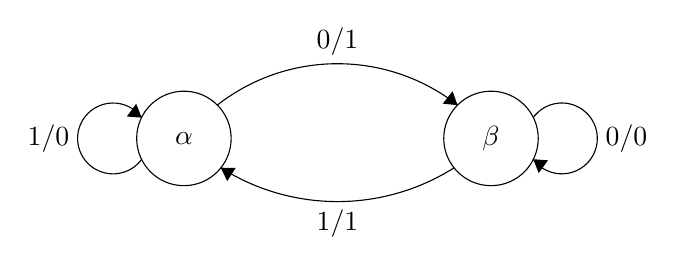
\begin{tikzpicture}[scale=0.2]
\tikzstyle{every node}+=[inner sep=0pt]
\draw [black] (15.8,-29.2) circle (3);
\draw (15.8,-29.2) node {$\alpha$};
\draw [black] (35.3,-29.2) circle (3);
\draw (35.3,-29.2) node {$\beta$};
\draw [black] (13.12,-30.523) arc (-36:-324:2.25);
\draw (8.55,-29.2) node [left] {$1/0$};
\fill [black] (13.12,-27.88) -- (12.77,-27) -- (12.18,-27.81);
\draw [black] (17.918,-27.085) arc (128.02449:51.97551:12.39);
\fill [black] (33.18,-27.09) -- (32.86,-26.2) -- (32.24,-26.99);
\draw (25.55,-23.96) node [above] {$0/1$};
\draw [black] (37.98,-27.877) arc (144:-144:2.25);
\draw (42.55,-29.2) node [right] {$0/0$};
\fill [black] (37.98,-30.52) -- (38.33,-31.4) -- (38.92,-30.59);
\draw [black] (32.957,-31.065) arc (-57.68311:-122.31689:13.856);
\fill [black] (18.14,-31.06) -- (18.55,-31.91) -- (19.09,-31.07);
\draw (25.55,-33.71) node [below] {$1/1$};
\end{tikzpicture}
\end{center}

Here we represent the transition function $\tau$ graphically by showing
an edge $a/b$ from $s_1$ to $s_2$ exactly when $\tau(s_1,a) = (s_2,b)$.
So $\alpha$ is a Toggle State, $\beta$ is a Copy State, 
$\del_0 \underline{\alpha} = \underline{\beta}$, 
and $\del_1 \underline{\alpha} = \underline{\alpha}$.
Further,
$\underline{\alpha}(011) = 1\underline{\beta}11 = 11\underline{\alpha}1 = 110$.

Somewhat surprisingly, $\G(\A)$ is already the lamplighter group, 
$\Z/2\Z \wr \Z$ \cite{GrigorchukZuk01:lamplighter}, and classifying the
groups generated by automata of low state complexity is still an open problem
[references].
For a more in depth description of Mealy Automata and their properties, 
see \cite{Holcombe, Sakarovitch09:automata_theory}.


\subsection{Abelian Automata}
We restrict ourselves to the case where $\G(\A)$ is abelian, 
and use methods of Nekrashevich and Sidki to characterize these groups.
Further, we restrict ourselves to morphisms which additionally preserve 
the residuation structure, as this is responsible for the interesting 
structure of these groups ($\G(\A)$ is abelian if and only if it is 
either torsion free abelian or boolean 
\cite{NekrashevychSidki04:automorphisms}). We will use additive 
notation for our groups, and $I$ will denote the identity element. An
automaton is called \textbf{Trivial} iff its group is $\{ I \}$.
It is a theorem by Sutner \cite{Sutner18:abelian_automata} 
that $\G(\A)$ is abelian iff for even states $\del_0 f - \del_1 f = I$ 
and for odd states $\del_1 f - \del_0 f = \gamma$, where $\gamma$ is 
independent of $f$. Moreover, the case $\gamma = I$ corresponds 
precisely to the case where $\G(\A)$ is boolean.

We now restrict ourselves further to the case where $\G(\A)$ is 
free abelian, that is to say $\G(\A) \cong \Z^m$ for some $m$,
and $\gamma \not = I$.%
\footnote%
{%
  For historical reasons we use $\Z^m$ instead of $\Z^n$ because 
  traditionally $n$ is reserved for the size of the state set of 
  an automaton.
}
It was shown by Nekrashevich and Sidki 
\cite{NekrashevychSidki04:automorphisms} 
that $\Z^m$ itself can be considered the state set of an invertible transducer.
The odd (resp. even) states are exactly the vectors with odd (resp. even) 
first component. To define the transition function, we require a 
$\frac{1}{2}-integral$ matrix $\Am$ of $\Q$-irreducible character. 
To ensure that the group is generated by \emph{finite} state machines, we 
require $\Am$ to be a contraction. That is, all of its complex eigenvalues 
should have norm $<1$. By $\frac{1}{2}-integral$, we mean a matrix of the
form

\[
\begin{pmatrix}
  \frac{a_{11}}{2} & a_{12} & \dots  & a_{1n}\\
  \vdots           & \vdots & \ddots & \vdots\\
  \frac{a_{n1}}{2} & a_{n2} & \dots  & a_{nn}\\
\end{pmatrix}
\]

where each $a_{ij} \in \Z$. These matrices all have characteristic polynomial
$\chi = x^n + \frac{1}{2}g(x)$, where $g \in \Z[x]$ and has constant term 
$\pm 1$.\\ 
Note $\Am : 2\Z \oplus \Z^{m-1} \to \Z^m$.
Thus we can define residuation as multiplication by $\Am$ for even vectors,
but for odd vectors we need to first make them even. To that end, let $\e$
be odd, and define residuation as follows:

If $\v$ is even:
\[ \del_0 \v = \del_1 \v = \Am \v \]

If $\v$ is odd:
\[ \del_0 \v = \Am (\v - \e) \]
\[ \del_1 \v = \Am (\v + \e) \]
Following Sutner \cite{Sutner18:abelian_automata}, we call this 
\textbf{The Complete Automaton} $\C$. 

Nekrashevich and Sidki proved that every torision free abelian 
group $\G(\A)$ is isomorphic to $\C$ for some $\Am$ and $\e$ 
\cite{NekrashevychSidki04:automorphisms} and $\A$ is a natural 
subautomaton of this machine if we identify $s \in \A$ with 
$\underline{s} \in \G(\A)$. While $\Am$ is easily seen to be unique
up to GL($\Q$) similarity, there are infinitely many valid choices for
$\e$, and classifying these is a major point of this paper. However, one
always exists, and going forward we will identify $\G(\A)$ with an 
appropriately chosen $\C$. Since this choice is somwhat arbitrary,
we say a function $f \in \G(\A)$ is \textbf{Located at} $\v \in \C$ iff
the isomorphism between $\G(\A)$ and $\C$ sends $f$ to $\v$. 
Further, given any state $\v \in \C$, closing $\{ \v \}$ under residuation 
will result in a finite automaton $\A_{\v}$ since $\Am$ is a contraction.
So we say an automaton $\A$ is \textbf{Located At} $\v \in \C$ iff the
isomorphism sends $\A$ to $\A_{\v} \subseteq \C$. Note that the location of a 
function or an automaton, and indeed whether a location exists or not, will 
depend on the choice of $\e$.

\subsection{Principal Automata}
It was shown by Okano \cite{Okano15:thesis} that there is a 
distinguished automaton, now called the \textbf{Principal Automaton} $\P$, 
associated to each matrix. $\P(\Am)$ is defined to be 
$\P = \A_{\e_1} \cup \A_{-\e_1} \subseteq \mathfrak{C}(\Am, \e_1)$,
though there is a longstanding conjecture that in most cases this is
the same machine as $\A_{\e_1} \subseteq \mathfrak{C}(\Am, \e_1)$.
We will write $\P$ when the matrix is clear from context. 

We shall soon see that $\P$ is located at $\e$ in $\C$ for all $\e$,
and so we call this group element $\delta \in \G(\P)$. Notice that for
all $\e$, $\del_0 \delta = \Am(\e - \e) = \bar{0} = I$, and so
$\del_1 \delta = \gamma$, since for any odd vector 
$\del_1 \v - \del_0 \v = \gamma$.

$\P$ is clearly minimal in terms of state complexity, as its states are
distinct group elements of $\mathfrak{C}(\Am, \e_1)$ and therefore 
definitionally have different behavior. However, $\P$ is minimal in the
subgroup relation for nontrivial automata sharing its matrix. 
While there are proofs of this claim which rely heavily on the
ambient linear algebraic structure \cite{Okano15:thesis}, 
we present here a difference construction which uses only the given 
automaton $\A$ to construct $\P$.

\begin{thm}
  For each nontrivial $\A$ with associated matrix $\Am$,\\
  $\G(\P(\Am)) \leq \G(\A)$.
\end{thm}

\begin{proof}
  Let $\A$ be an abelian automaton with at least one odd state.
  Note that if $\A$ has no odd states, its group is trivial, so we may
  safely ignore it.

  Put $\gamma = \del_1 f - \del_0 f$ for $f \in \A$ odd, and construct
  a new automaton by closing $\gamma$ under residuation.

  Note that this can be done using only information contained in $\A$,
  since it is easy to check that:
  \[
    \del_0(f + g) = \begin{cases} \del_0 f + \del_1 g & \text{both odd}\\
                                  \del_0 f + \del_0 g & \text{otherwise}
                    \end{cases}
  \]
  \[
    \del_1(f + g) = \begin{cases} \del_1 f + \del_0 g & \text{both odd}\\
                                  \del_1 f + \del_1 g & \text{otherwise}
                    \end{cases}
  \]
  \[
    \del_0 (-f) = - \del_1 f
  \]
  \[
    \del_1 (-f) = - \del_0 f
  \]

  Thus using the characterization by Sutner \cite{Sutner18:abelian_automata}, 
  that a state is odd iff it has distinct residuals, we can close $\gamma$ 
  under residuation by looking only at $\A$.
  Since $\gamma \in \G(\A)$ and $\G(\A)$ is residuation closed, 
  this entire closure is a subset of $\G(\A)$. 

  Now, if necessary, we can join this automaton with its negation, and
  possibly add states $\delta$ and $-\delta$ residuating into $I$
  (an even self loop) and $\pm \gamma$ to construct 
  $\P(\Am) \subseteq \G(\A)$. Then $\G(\P(\Am)) \leq \G(\A)$, as desired.
\end{proof}

\subsection{An Example}
Consider the following machine, $\A^3_2$:

\begin{center}
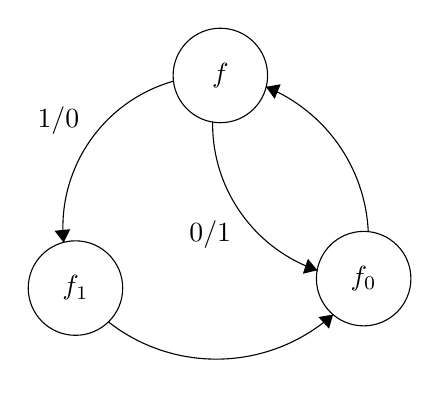
\begin{tikzpicture}[scale=0.2]
\tikzstyle{every node}+=[inner sep=0pt]
\draw [black] (26.6,-12.1) circle (3);
\draw (26.6,-12.1) node {$f$};
\draw [black] (17.4,-25.6) circle (3);
\draw (17.4,-25.6) node {$f_1$};
\draw [black] (35.7,-25) circle (3);
\draw (35.7,-25) node {$f_0$};
\draw [black] (16.648,-22.708) arc (-174.31762:-254.2298:9.658);
\fill [black] (16.65,-22.71) -- (17.07,-21.86) -- (16.07,-21.96);
\draw (17.67,-14.97) node [left] {$1/0$};
\draw [black] (33.761,-27.277) arc (-48.14861:-128.09563:11.117);
\fill [black] (33.76,-27.28) -- (32.83,-27.44) -- (33.5,-28.18);
\draw [black] (29.501,-12.822) arc (67.8011:2.5992:10.451);
\fill [black] (29.5,-12.82) -- (30.05,-13.59) -- (30.43,-12.66);
\draw [black] (32.758,-24.474) arc (-108.88288:-180.71682:9.832);
\fill [black] (32.76,-24.47) -- (32.16,-23.74) -- (31.84,-24.69);
\draw (27.31,-22.21) node [left] {$0/1$};
\end{tikzpicture}
\end{center}

Here the unlabeled transitions both copy the input bit, however these
have been omitted for cleanliness.

Then we can construct the principal machine as follows:

\begin{center}
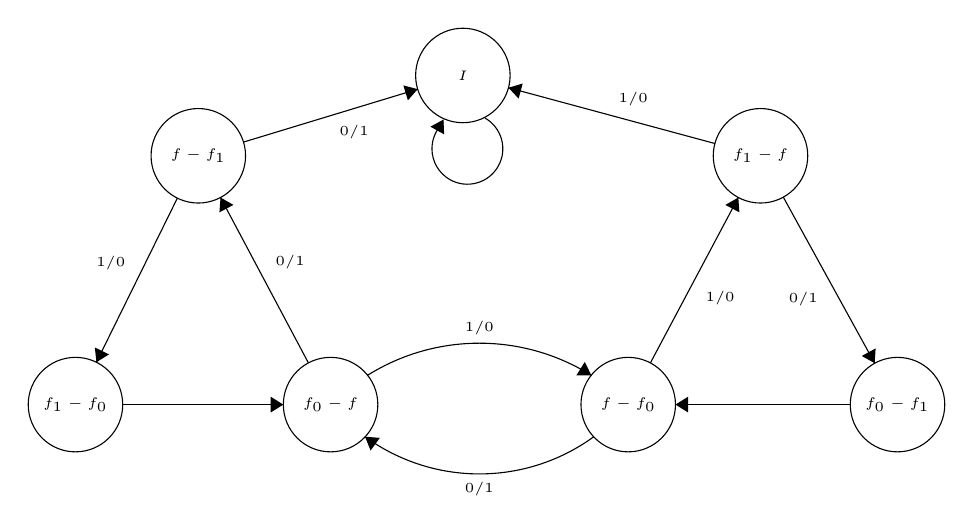
\begin{tikzpicture}[scale=0.2]
\tikzstyle{every node}+=[inner sep=0pt]
\draw [black] (36.4,-15.9) circle (3);
\draw (36.4,-15.9) node {\tiny $I$};
\draw [black] (37.8,-18.6) arc (60.34019:-227.65981:2.25);
\fill [black] (35.17,-18.7) -- (34.34,-19.15) -- (35.21,-19.64);
\draw [black] (55.3,-21) circle (3);
\draw (55.3,-21) node {\tiny $f_1-f$};
\draw [black] (64,-36.8) circle (3);
\draw (64,-36.8) node {\tiny $f_0-f_1$};
\draw [black] (46.9,-36.8) circle (3);
\draw (46.9,-36.8) node {\tiny $f-f_0$};
\draw [black] (28,-36.8) circle (3);
\draw (28,-36.8) node {\tiny $f_0-f$};
\draw [black] (11.8,-36.8) circle (3);
\draw (11.8,-36.8) node {\tiny $f_1-f_0$};
\draw [black] (19.6,-21) circle (3);
\draw (19.6,-21) node {\tiny $f-f_1$};
\draw [black] (22.47,-20.13) -- (33.53,-16.77);
\fill [black] (33.53,-16.77) -- (32.62,-16.53) -- (32.91,-17.48);
\draw (29.5,-19.03) node [below] {\tiny $0/1$};
\draw [black] (18.27,-23.69) -- (13.13,-34.11);
\fill [black] (13.13,-34.11) -- (13.93,-33.61) -- (13.03,-33.17);
\draw (15,-27.81) node [left] {\tiny $1/0$};
\draw [black] (14.8,-36.8) -- (25,-36.8);
\fill [black] (25,-36.8) -- (24.2,-36.3) -- (24.2,-37.3);
\draw [black] (26.59,-34.15) -- (21.01,-23.65);
\fill [black] (21.01,-23.65) -- (20.94,-24.59) -- (21.83,-24.12);
\draw (24.48,-27.74) node [right] {\tiny $0/1$};
\draw [black] (30.345,-34.939) arc (122.03013:57.96987:13.397);
\fill [black] (44.56,-34.94) -- (44.14,-34.09) -- (43.61,-34.94);
\draw (37.45,-32.4) node [above] {\tiny $1/0$};
\draw [black] (52.4,-20.22) -- (39.3,-16.68);
\fill [black] (39.3,-16.68) -- (39.94,-17.37) -- (40.2,-16.41);
\draw (47.22,-17.84) node [above] {\tiny $1/0$};
\draw [black] (56.75,-23.63) -- (62.55,-34.17);
\fill [black] (62.55,-34.17) -- (62.61,-33.23) -- (61.73,-33.71);
\draw (58.98,-30.09) node [left] {\tiny $0/1$};
\draw [black] (61,-36.8) -- (49.9,-36.8);
\fill [black] (49.9,-36.8) -- (50.7,-37.3) -- (50.7,-36.3);
\draw [black] (48.31,-34.15) -- (53.89,-23.65);
\fill [black] (53.89,-23.65) -- (53.07,-24.12) -- (53.96,-24.59);
\draw (51.78,-30.06) node [right] {\tiny $1/0$};
\draw [black] (44.711,-38.841) arc (-53.966:-126.034:12.343);
\fill [black] (30.19,-38.84) -- (30.54,-39.72) -- (31.13,-38.91);
\draw (37.45,-41.7) node [below] {\tiny $0/1$};
\end{tikzpicture}
\end{center}

It is easy to check that this is the principal machine for
$\Am = \begin{pmatrix} -1 & 1 \\ -\frac{1}{2} & 0 \end{pmatrix}$,
and further that $\A^3_2$ as above is located at 
$\e_1 \in \mathfrak{C}\left ( \Am, \begin{pmatrix} 3 \\ 2 \end{pmatrix} \right )$

Notice that in this case we did not need to explicitly add the 
inverse machine, or indeed $\pm \delta$. The Strongly Connected Component
Conjecture states that this will be the case whenever $\Am$ has 
characteristic polynomial other than $x^m - \frac{1}{2}$, which corresponds
to the so called sausage automata. Unfortunately, however, 
this conjecture is yet unproven.

\section{Group Extensions}
Going forward, $\G$ will denote $\G(\P)$ for some principal machine $\P$.

$\G$ clearly admits representation as a $\Z[x]$ module where 
$x \cdot \v = \Am^{-1}\v$, extended linearly. Further, since $\Am$ has 
irreducible character so does $\Am^{-1}$. Thus this module is cyclic, 
and generated by $\e_1 = \delta$. 
(Note that since $\Am$ sends $2\Z \oplus \Z^{m-1}$ to $\Z^m$, and therefore
has multiples of $\frac{1}{2}$ in general, $\Am^{-1}$ sends $\Z^m$ to 
$2\Z \oplus \Z^{m-1}$, and so has only integer entries).

Clearly $\text{End}_{\G}$, the ring of module endomorphisms of $\G$, 
is isomorphic to $\Z[x]/(\chi^*)$, 
where $\chi^*$ is the characteristic polynomial of $\Am^{-1}$.
Now for some $p \in \text{End}_{\G}$ we write
$p \cdot \G$ in place of $\G(\mathfrak{C}(\Am,p \cdot \e_1))$.
That is to say, $p \cdot \G$ has as its states $\Z^m$ and as its 
odd residuations
$\del_0 \v = \Am (\v - p \cdot \e_1)$, and 
$\del_1 \v = \Am (\v + p \cdot \e_1)$

Since the residuation vector must be odd, we note $p$ must have odd
constant term. Further, since this module is cyclic, every $\v$ arises as 
$p_{\v} \cdot \e_1$ where $p_{\v} = \v_0 + \v_1 x + \ldots + \v_{m-1} x^{m-1}$.

For reasons which will soon become clear, we call $p \cdot \G$ the
\textbf{Group Extension} of $\G$ by $p$.

To justify this nomenclature, we first notice 
$\G \hookrightarrow p \cdot \G$ for all $p$ by the
homomorphism $\v \mapsto p \cdot \v$. 
Further, we recognize that if $p$ is not a unit in $\text{End}_{\G}$, 
this homomorphism is \emph{not} surjective. 
That is to say $\G$ is a proper subgroup of $p \cdot \G$.
This observation is true in higher generality, as shown below.

\begin{thm}
  If $rp = q$ in $\Z[x]$, then $p \cdot \G \hookrightarrow q \cdot \G$, 
  with a canonical injection $\varphi_r~:~\v \mapsto r \cdot \v$. 
  In particular, if $r$ is a unit, then $p \cdot \G \cong q \cdot \G$.
\end{thm}

\begin{proof}
  Let $rp = q$, $f \in p \cdot \G$ located at $\v$.
  Consider $f' \in q \cdot \G$ located at $r \cdot \v$.

  First note $f$ and $f'$ have the same parity, since 
  $r$ has odd constant term, and so $\v$ and $r \cdot \v$
  have the same parity. Now, consider the residuals of $f$ and $f'$. 
  
  If $f$ is even, then 
  \[ \del_0 f' = \Am (r \cdot \v) = r \cdot \Am \v = r \cdot \del_0 f \]

  If $f$ is odd, then
  \[ \del_0 f' = \Am (r \cdot \v - q \cdot \e_1) 
               = r \cdot \Am (\v - p \cdot \e_1)
               = r \cdot \del_0 f \]

  A similar argument shows $\del_1 f' = r \cdot \del_1 f$
\end{proof}

\section{Fractional Elements}
For a vector $p \cdot \v$ in $p \cdot \G$, we are working with exactly
the functions already present in $\G$. However, most vectors cannot be written
as $p \cdot \v$. What do they do as functions?
We call such vectors (and their corresponding functions)
\textbf{Fractional}, due to the following observation and theorem.

Consider $\e_1 \in 3 \cdot \G$. By the above theorem, $3\e_1 = \delta$,
and so we should expect $\e_1$ to behave like ``$\frac{1}{3}\delta$'', 
and in fact it does.

In general, $\v \in p \cdot \G$ behaves like $p^{-1} \cdot \v \in \G$,
(where $p^{-1}$ comes from $\Q[x]$ and so $p^{-1} \cdot \v \in \Q^m$)
and so Group Extensions give us access to fractional functions from 
our base group $\G$.

\begin{thm}
  For $p \in Z[x]$ with odd constant term, 
  $p^{-1} \cdot \Z^m \cong p \cdot \G$.
\end{thm}

\begin{proof}
  Here we think of $p^{-1} \cdot \Z^m = \{ p^{-1} \cdot \v~|~\v \in \Z^m \}$
  as a subgroup of $\Q^m$. Residuation in this setting is given by
  $\del_0 \v = \Am (\v - \e_1)$ and $\del_1 \v = \Am (\v + \e_1)$ 

  Consider $\varphi~:~p^{-1} \cdot \Z^m \to p \cdot \G$ by
  $\varphi(p^{-1} \cdot \v) = \v$.\\
  $\varphi$ is clearly bijective, and is a homomorphism since:
  \begin{align*}
       \varphi(p^{-1} \cdot \v_1 + p^{-1} \cdot \v_2) 
    &= \varphi(p^{-1} \cdot (\v_1 + \v_2))\\
    &= \v_1 + \v_2\\
    &= \varphi(p^{-1} \cdot \v_1) + \varphi(p^{-1} \cdot \v_2) 
  \end{align*}

  Further, if $\v$ is even, then:

  \begin{align*}
       \varphi(\del_0 p^{-1} \cdot \v)
    &= \varphi(\Am p^{-1} \cdot \v)\\
    &= \varphi(p^{-1} \cdot \Am \v)\\
    &= \Am \v\\
    &= \del_0 \varphi(p^{-1} \cdot \v)
  \end{align*}

  If $\v$ is odd, then: 

  \begin{align*}
       \varphi(\del_0 p^{-1} \cdot \v)
    &= \varphi(\Am (p^{-1} \cdot \v - \e_1))\\
    &= \varphi(p^{-1} \cdot \Am (\v - p \cdot \e_1))\\
    &= \Am (\v - p \cdot \e_1)\\
    &= \del_0 \varphi(p^{-1} \cdot \v)
  \end{align*}

  The proof for $\del_1$ is similar.
\end{proof}

Thus we can view functions in $p \cdot \G$ as fractions of functions in $\G$.
It is a natural question to ask which fractions are attainable in this way.

Clearly, for any $f \in \G$, we can attain $\frac{1}{k} f$ for any odd $k$.
Simply take $\v \in k \cdot \G$ for $f$ located at $\v$.
However, fractions with even denominator are unattainable.
$2 \frac{1}{2}\delta = \delta$ should be an odd function,
but no function, when doubled, is odd.

\section{Characterizing Automata}
Since each automaton $\A$ is a subautomaton of some $\C$,
equivalently some $p \cdot \G$, there should be a minimal $\e$ 
(up to multiplication by units) which still has $\A$ as a subautomaton. 

Notice that if we locate $\A$ at $\e_1 \in p \cdot \G$, 
then there can be no smaller polynomial $q$ (in the division ordering)
which also places $\A$ at an integral position, because, by the above
theorems:\\ 
$\e_1 \in p \cdot \G$ is located at $p^{-1}q \cdot \e_1 \in q \cdot \G$, 
and $p^{-1}q \cdot \e_1$ is fractional.


\begin{thm}
  Every nontrivial abelian automaton $\A$ can be 
  located at $\e_1$ in $p \cdot \G$ for some $p$.
\end{thm}

\begin{proof}
  It is a theorem by Sutner \cite{Sutner18:abelian_automata} that every 
  abelian automaton residuates into a strongly connected component, 
  and further that this component generates the same group as the entire 
  machine. So we may, with no loss of generality, assume our machine is 
  strongly connected (that is, every state except possibly $I$ has a path to
  every other state).

  Let $f$ be an odd state in $\A$. Then at least one of $\del_0 f$ and 
  $\del_1 f$ is not equal to $f$. Then there is some nontrivial cycle
  from $f$ to itself, which we can represent by a matrix equation 
  relating $\v_f$, and $\e$. (Here $\v_f$ is where $f$ will be located, 
  and $\e$ will be the eventual residuation vector). 
  We can then rearrange this equation to obtain 
  $p_1(\Am)\v_f = p_2(\Am)\e$.

  However, $p_1, p_2 \in \Z[x]$ but $\Am$ has irreducible character over $\Z$.
  It is well known that the eigenvalues of $p(\Am)$ are precisely $p(\lambda)$
  where $\lambda$ is an eigenvalue of $\Am$, so $\Am$'s invertibility implies
  the invertibility of both $p_1$ and $p_2$. Thus

  \[ \e = p_2(\Am)^{-1}p_1(\Am)\v_f \]

  Choosing $\v_f = \e_1$ gives a value for the residuation vector $\e$,
  which (by cyclicity) gives a polynomial $p_e$ 
  such that $p_e \cdot \e_1 = \e$. Then, by construction, $\A$ is 
  a subautomaton of $p_e \cdot \G$, and is anchored with $f$ at $\e_1$.
  As desired.
\end{proof}

Then for any automaton $\A$, we can now completely characterize in
which complete machines it can be located, and at what vectors.
Simply locate $\A$ at $\e_1 \in p \cdot \G$, and then to locate it at
any odd vector $\v$, scale both sides by $p_{\v}$ to see $\A$ located at
$\v \in p_{\v} p \cdot \G$.

Further, given some polynomial $q$, $\A$ is located somewhere in $q$ 
if and only if $p \mid q$. Further, it will be located at 
$p^{-1}q \cdot e_1$.

\subsection{An Example}

Recall the abelian automaton $\A^3_2$ from earlier in the paper:

\begin{center}
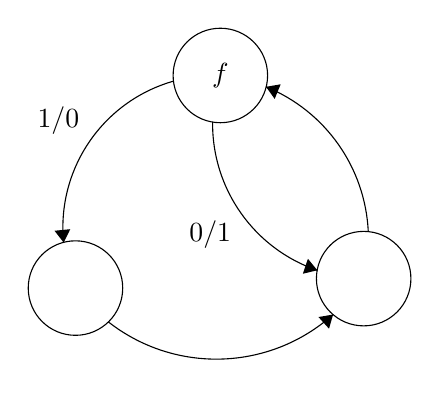
\begin{tikzpicture}[scale=0.2]
\tikzstyle{every node}+=[inner sep=0pt]
\draw [black] (26.6,-12.1) circle (3);
\draw (26.6,-12.1) node {$f$};
\draw [black] (17.4,-25.6) circle (3);
\draw [black] (35.7,-25) circle (3);
\draw [black] (16.648,-22.708) arc (-174.31762:-254.2298:9.658);
\fill [black] (16.65,-22.71) -- (17.07,-21.86) -- (16.07,-21.96);
\draw (17.67,-14.97) node [left] {$1/0$};
\draw [black] (33.761,-27.277) arc (-48.14861:-128.09563:11.117);
\fill [black] (33.76,-27.28) -- (32.83,-27.44) -- (33.5,-28.18);
\draw [black] (29.501,-12.822) arc (67.8011:2.5992:10.451);
\fill [black] (29.5,-12.82) -- (30.05,-13.59) -- (30.43,-12.66);
\draw [black] (32.758,-24.474) arc (-108.88288:-180.71682:9.832);
\fill [black] (32.76,-24.47) -- (32.16,-23.74) -- (31.84,-24.69);
\draw (27.31,-22.21) node [left] {$0/1$};
\end{tikzpicture}
\end{center}

Say we want to find $\v$ and $\e$ such that $\A^3_2$ is located at 
$\v \in \C$.

Using the algorithm described by Becker gives 
$\Am = \begin{pmatrix} -1 & 1 \\ -\frac{1}{2} & 0 \end{pmatrix}$.

Then notice $\del_0 \del_0 f = f$.
So $\Am^2 (\v_f - \e) = \v_f$, and
$\Am^2 \v_f - \v_f = \Am^2 \e$. Thus

\[ \e = \Am^{-2} (\Am^2 - I) \v_f \]

Choosing $\v_f = \e_1$ gives $\e = \begin{pmatrix} 3 \\ 2 \end{pmatrix}$.

Then $f = \begin{pmatrix} 1 \\ 0 \end{pmatrix} \in (3+2x) \cdot \G$

\subsection{Limiting Objects}
Since each $p \cdot \G$ can be viewed as $p^{-1} \cdot \Z^m \subseteq \Q^m$,
with residuation vector $\e$ given consistently by $\e_1$,
it is reasonable to consider the subgroup of $\Q^m$
\[ 
  \widetilde{\G} = \bigcup_p p^{-1} \cdot \Z^m 
\]
(Recall we only include polynomials with odd constant term in this union)

Notice that this group is universal, in the sense that it contains as
subgroups each $p \cdot \G$. Further, it concretely shows the relationships
between the various automata. In this group, each automaton $\A$ with
the correct matrix is located at exactly one vector, namely 
$p^{-1} \cdot \e_1$ where $p$ is the polynomial such that $\A$ is located
at $\e_1 \in p \cdot \G$.

In fact, in this setting, we see exactly why automata show up in multiple
group extensions, and why the division ordering of polynomials is the 
characterizing factor. $p \cdot \G$ is precisely $p \cdot \widetilde{\G}$, 
where residuation is necessarily scaled up, and we look at only integer
vectors.

\section{Characterizing Orbits}

Recall an \textbf{Orbit} of $f \in \G(\A)$ at $u \in \2^{\omega}$
is $\{ f^t u~|~t \in \Z \}$, or, additively, $\{ tf u~|~t \in \Z \}$.
It is a reasonable question to wonder what these orbits look like
for an arbitrary function $f$. We will soon see they look like lines
with slope $f$ and ``intercept'' given by $\langle u \rangle$, which sends
$0^{|u|}$ to $u$.

We begin with a useful lemma: we can flip just the ith bit.

\begin{thm}
  $(x^n \cdot \delta) (u0v) = u1v$ 
  (when $|u| = n$, and $v \in \2^*$ or $\2^\omega$)
\end{thm}

\begin{proof}
  If $n=0$ the theorem is clear, since 
  $\delta 0v = 1 (\del_0 \delta v) = 1 (I v) = 1v$

  Further, $\Am^{-1}f$ is always even 
  (since $\Am^{-1}:2\Z \oplus \Z^{m-1}$), 
  and so copies the first bit, then applies $f$. 
  The claim follows by induction.

\end{proof}

We will first prove the result in the finite case.

\begin{thm}
  For every word $u \in \2^n$, there exists a unique function
  (mod $Stab(0^n)$) sending $0^n$ to $u$. Following Sutner and Lewi
  \cite{SutnerLewi12:iter_inver_bin_trans}, we call this function
  $\langle u \rangle$.
\end{thm}

\begin{proof}
  The existance of such a function is a direct consequence of the lemma,
  and is given by $\sum_{i=0}^{n-1} u_i x^i \delta$.
  Uniqueness mod $Stab(0^n)$ is immediate.
\end{proof}

\begin{thm}
  The orbit of $f$ at $u$ is given by the line $\Z f + \langle u \rangle$
\end{thm}

\begin{proof}
  Let $w = tf u$ be in the orbit of $u$. Then $\langle w \rangle$ sends 
  $0^n$ to $w$, but so does $tf + \langle u \rangle$. By uniqueness, then,
  $\langle w \rangle = tf + \langle u \rangle$ and the theorem follows.
\end{proof}

Note that this argument works in the infinite case as well 
(it arguably works better, since Stab($0^\omega$) is trivial), though
the obvious extension $\langle u \rangle = \sum_{i=0}^{\infty} u_i x^i \delta$ 
for $u \in \2^\omega$ cannot be effective in general for cardinality reasons. 
We clearly cannot send $0^\omega$ to any $u$ without working in the 
topological closure $\widehat{\G}$, where we may lose finiteness of our 
automata. Further, since every $f$ residuates into a strongly connected 
component, every $f$ sends $0^\omega$ to an ultimately periodic string.
This is the only obstruction.

\begin{thm}
  For $u \in \2^\omega$, $\langle u \rangle$ exists in some group extension
  iff $u$ is ultimately periodic.
\end{thm}

\begin{proof}
  Since every function $f \in p \cdot \G$ eventualy residuates into a finite
  strongly connected component, $f 0^\omega$ is ultimately periodic for
  every such $f$.

  Further, if we have an ultimately periodic string $u = tv^{\omega}$, then
  $\sum_{i=0}^{\infty} u_i x^i \delta$ works if it exists in some group 
  extension. It does, since:

  \begin{align*}
    \sum_{i=0}^{\infty} u_i x^i \delta 
    &= \left ( 
        \sum_{i=0}^{|t|} t_i x^i
        + x^{|t|} \frac{\sum_{i=0}^{|v|} v_i x^i}{1 - x^{|v|}}
       \right ) \cdot \delta\\
    &= \frac%
        {%
          \left ( 1 - x^{|v|} \right ) \sum_{i=0}^{|t|} t_i x^i + 
          x^{|t|} \sum_{i=0}^{|v|} v_i x^i
        }
        {1 - x^{|v|}}
       \cdot \delta\\
  \end{align*}

  This last sum is of the form $\frac{q}{1 - x^{|v|}} \cdot \delta$, 
  Thus, this sum is equal to $q \cdot \delta \in (1 - x^{|v|}) \cdot \G$.
  (Or, equivalently, $\frac{q}{1 - x^{|v|}} \cdot \delta \in \widetilde{\G}$)
\end{proof}

\section{Conclusion}
We have shown what the residuation vector $\e$ means with respect to the
complete automata, and additionally have shown the existance of a limit
object which removes the need for this parameter, with no loss of information.
Finally we used inspiration from a paper by Sutner and Lewi 
\cite{SutnerLewi12:iter_inver_bin_trans} to characterize
orbits for $\2^*$ and $\2^\omega$, and characterize which of the $\2^\omega$
orbits are effective (the ultimately periodic strings).

Further, the existence of the universal object $\widetilde{\G}$ sheds new light
on the connection between affine tiles 
\cite{LagariasWang96:tiles, LagariasWang97:integral_tiles}
and abelian automata noted by Sutner
\cite{Sutner18:abelian_automata}. Indeed it is easy to see that in 
$\widetilde{\G}$ every strongly connected component 
(and thus every subautomaton of interest) has each vector in the attractor 
of the iterated function system given by the residuation functions 
$\{ \v \mapsto \Am \v, \v \mapsto \Am (\v \pm \e_1) \}$.
Thus, in particular, the size of the principal machine is bounded by the
number of integral points in this attractor. 

The module theory discussed in this paper also provides a new take on a
proof technique for a longstanding conjecture referenced earlier in the paper,
called the Strongly Connected Component (SCC) Conjecture. This conjecture 
asserts that principal machines $\P$ have only one strongly connected component 
(plus the self looping identity state) whenever their matrix has a 
characteristic polynomial that is \emph{not} of the form $x^n + \frac{1}{2}$.
Sutner described Path Polynomials \cite{Sutner18:abelian_automata} which
allow us to reason about the existence of directed paths between states 
in an automaton by purely algebraic means. However, these polynomials were
clunky and not always defined. However, a different definition of path 
polynomial\footnote{%
  \begin{align*}
    P_\epsilon(x)   &= 1\\
    P_{w0}(x)       &= \Am^{-1}(P_w(x)) + 0\\
    P_{w1}(x)       &= \Am^{-1}(P_w(x)) + 1\\
    P_{w\bar{1}}(x) &= \Am^{-1}(P_w(x)) - 1
  \end{align*}
  Note the coefficients of $p_w$ encode the path from 
  $p_w \cdot \e_1$ to $e_1$ in a straightforward way,
  and if any $p_w = -1$ (mod $\chi^*$), 
  then there is a path from $-\e_1$ to $\e_1$, and,
  by symmetry, a path from $\e_1$ to $-\e_1$ as well. Thus $\P$ is
  generated by only $\e_1$.
}
, which moves \emph{backwards} along transitions 
instead of forwards, is always well defined, and is an element of 
$\text{End}_{\G}$. Then to prove the SCC conjecture, it suffices to prove 
that whenver $\Am$ does not have characteristic $x^n + \frac{1}{2}$
there is a polynomial $p \in \{-1,0,1\}[x]$ which is congruent to $-1$ mod
$\chi^*$. Efforts are underway to use this method to actually prove the 
conjecture.

\newpage

\bibliographystyle{plain}
\bibliography{bib}

\end{document}
